% *********************************************************************
% © 2021 Jeremy Sylvestre
%
% Permission is granted to copy, distribute and/or modify this document
% under the terms of the GNU Free Documentation License, Version 1.3 or
% any later version published by the Free Software Foundation; with no
% Invariant Sections, no Front-Cover Texts, and no Back-Cover Texts. A
% copy of the license is included in the appendix entitled “GNU Free
% Documentation License” that appears in the output document of this
% PreTeXt source code. All trademarks™ are the registered® marks of
% their respective owners.
%
% *********************************************************************

\newcommand*{\xmin}{-2}
\newcommand*{\xmax}{2}
\newcommand*{\ymin}{-1}
\newcommand*{\ymax}{4}

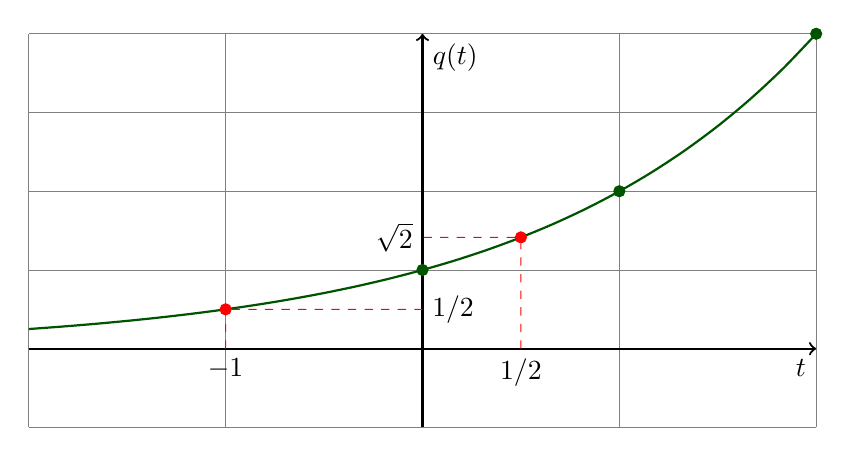
\begin{tikzpicture}
[
	closedpt/.style={circle,draw,fill,inner sep=0pt,minimum size=4pt},
	openpt/.style={circle,draw,inner sep=0pt,minimum size=4pt},
	xscale=2.5
]

	% grid
	\foreach \x in {\xmin,-1,0,...,\xmax} {
		\draw[very thin,gray] (\x,\ymin) -- (\x,\ymax);
	}
	\foreach \y in {\ymin,0,1,...,\ymax} {
		\draw[very thin,gray] (\xmin,\y) -- (\xmax,\y);
	}

	% label grid
	% \foreach \x in {1,2,3,4} {
	% 	\node[below] at (\x,0) {$\x$};
	% }
	% \foreach \y in {0.5,1} {
	% 	\node[left] at (0,\y) {$\y$};
	% }

	% axes
	\draw[->,thick] (\xmin,0) -- (\xmax,0) node[below left] {$t$};
	\draw[->,thick] (0,\ymin) -- (0,\ymax) node[below right] {$q(t)$};

	\draw[green!33!black,smooth,domain=-2:2,thick] plot (\x, {exp (0.693 * \x)});

	% data
	\node[green!33!black,closedpt] at (0,1) {};
	\node[green!33!black,closedpt] at (1,2) {};
	\node[green!33!black,closedpt] at (2,4) {};

	% new points
	\node[red,closedpt] at (-1,0.5) (recip) {};
	\node[red,closedpt] at (0.5,1.414) (root) {};
	\draw[red,dashed] (-1,0) -- (recip) -- (0,0.5);
	\draw[red,dashed] (0.5,0) -- (root) -- (0,1.414);

	\node[below] at (-1,0) {$-1$};
	\node[right] at (0,0.5) {$1/2$};

	\node[below] at (0.5,0) {$1/2$};
	\node[left] at (0,1.414) {$\sqrt{2}$};

\end{tikzpicture}
